\chapter{開発手法}
\label{chap:coding}

本章では DreamSacpe の概要、利用方法、システム概要について述べます。

\section{概観}
現在拡張現実に対する新しいアプローチの方法が求められている。本研究では睡眠中に思い出に関連した音を流すことで、その音に関連した夢を見ることを促進するスマートフォンアプリ、DreamScapeを提案する。DreamScapeでは記憶を思い起こさせる音声をコンテンツを、REM睡眠を感知した際に流すことで、ユーザーの夢を操作することを目指す。REM睡眠の感知はスマートフォンに備わっている加速度センサーを使用した。
 DreamScapeには3つの機能がある。一つ目は寝る前に印象に残っている記憶に関する写真と映像を表示する機能。二つ目は睡眠中にREM睡眠を検出し、記憶を連想させる音声を流す機能。最後に起床後に夢について記録する機能である。ユーザーには睡眠前にスマートフォンを図のように枕の横に置いてもらう。
 DreamScapeは開発途中でまだAppストアには掲示していないが、githubからソースコードを入手することができる。iOSスマートフォンを持っていて、Apple Developerの登録をしている人であればダウンロードできるようになっている。
\begin{figure}[htbp]
\begin{center}
\includegraphics[width=14cm]{eps/dreamDate02.eps}
\caption{DreamOnレビュー}
\label{DreamOnレビュー}
\end{center}
\end{figure}

\section{利用方法}
 DreamScapeを使うとき、ユーザーは事前に音声を登録してもらうことが必要となる。DreamScapeに適している音声と適さない音声がある。人の声、特に喋りかけてくるような内容の音声は、ユーザーを起こしてしまう可能性がある。適している音は繰り返しある環境下で聞いていた音である。例えば、旅で聞いていた曲、好きな映画のサウンドトラック、最寄り駅の音楽、特的の誰かと良く聞いていた音楽などが効果的だ。
 アプリの起動後、\ref{le01}のような画面が表示される。自動ロック機能をOFFにして、音量は1〜3に設定してもらう。 次にユーザーが登録した音楽が流れる。流れている最中はユーザーにできるだけ思い出の中の空間、香り、音をの細部をまで思い出して、気持ちを落ちつかせてもらう。ユーザーは寝る前にアプリを起動してスタートボタンを押し、起動させたままスクリーンを伏せて枕の横に置く。20〜30分間後にDreamScapeの加速度が起動をし、一晩中ユーザーの体動のモニタリングが行われ、REM睡眠を検知すると音楽がなる。
 起床後、ユーザーは起床すると夢の内容を忘れないように日記に投稿する。

\begin{figure}[htbp]
 \begin{minipage}{0.45\hsize}
  \begin{center}
   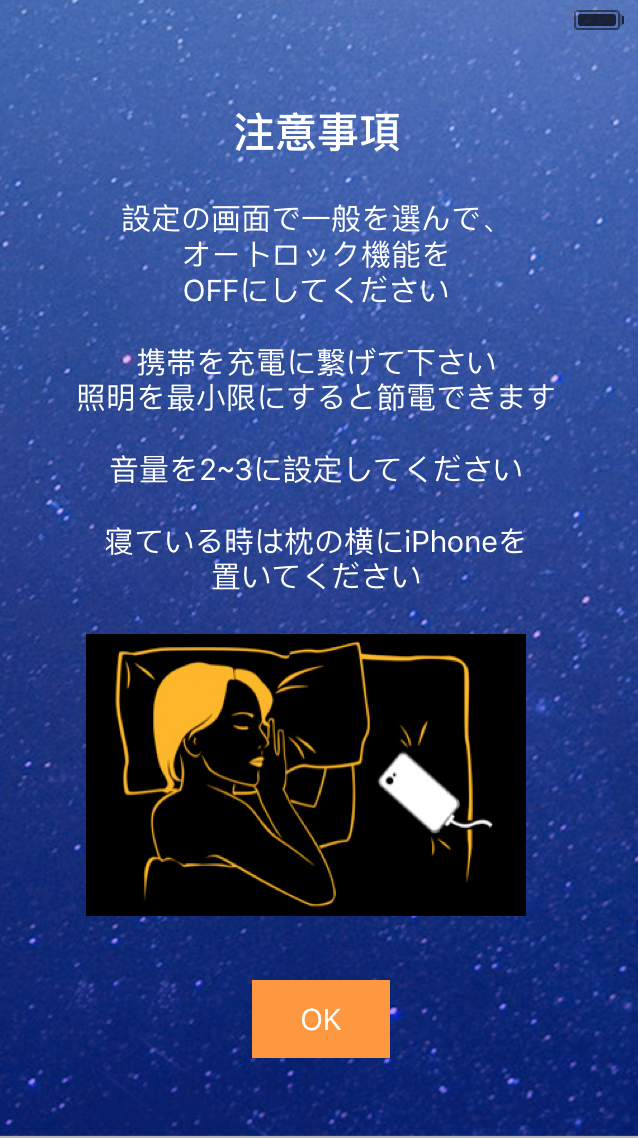
\includegraphics[height=90mm]{eps/AppIntro.eps}
  \end{center}
  \caption{起動画面}
  \label{le01}
 \end{minipage}
 \begin{minipage}{0.45\hsize}
  \begin{center}
   \includegraphics[height=90mm]{eps/AppMemoryImages.eps}
  \end{center}
  \caption{検索キーワードを入力}
  \label{le02}
 \end{minipage}
\end{figure}

\begin{figure}[htbp]
 \begin{minipage}{0.45\hsize}
  \begin{center}
   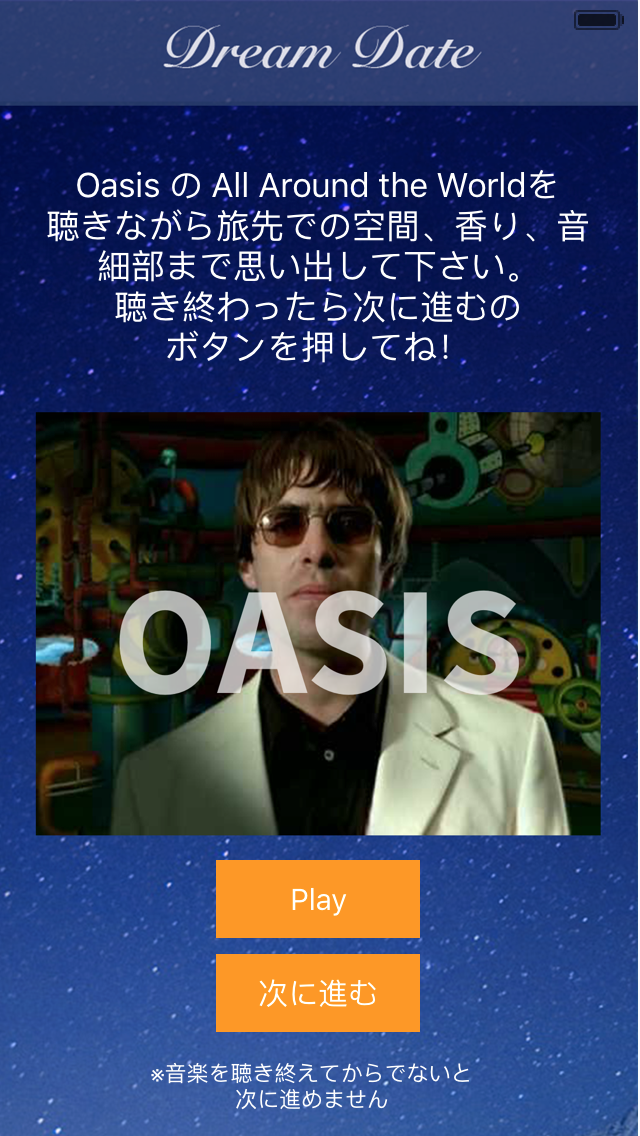
\includegraphics[height=90mm]{eps/AppMusicPlay.eps}
  \end{center}
  \caption{検索ボタンを押下}
  \label{le03}
 \end{minipage}
 \begin{minipage}{0.45\hsize}
  \begin{center}
   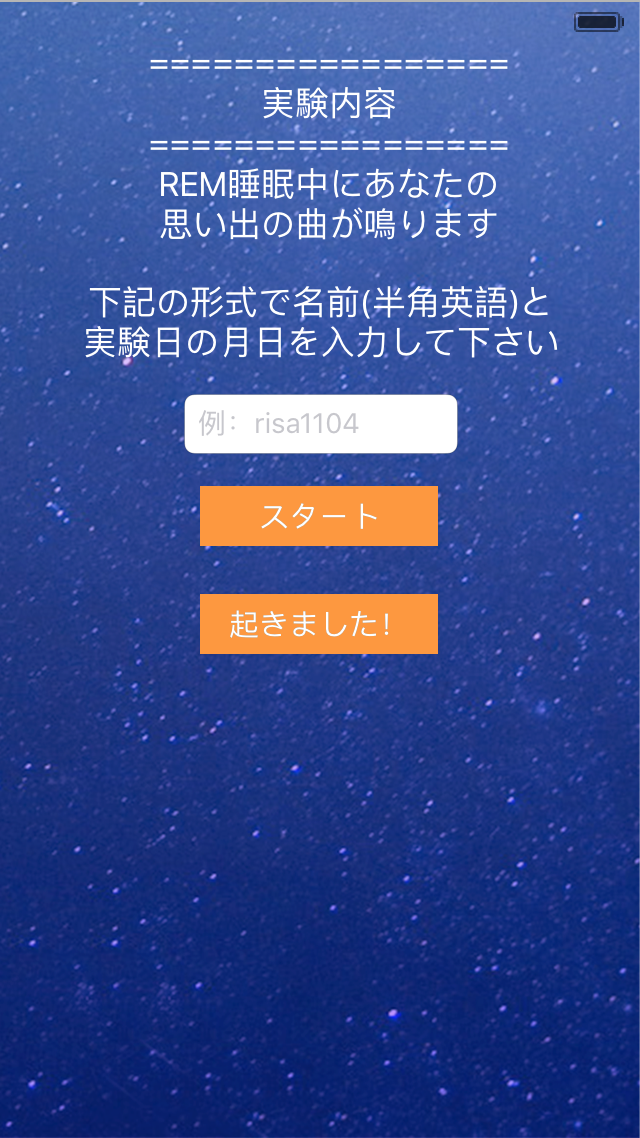
\includegraphics[height=90mm]{eps/AppStart.eps}
  \end{center}
  \caption{コンテンツ表示}
  \label{le04}
 \end{minipage}
\end{figure}

\begin{figure}[htbp]
 \begin{minipage}{0.45\hsize}
  \begin{center}
   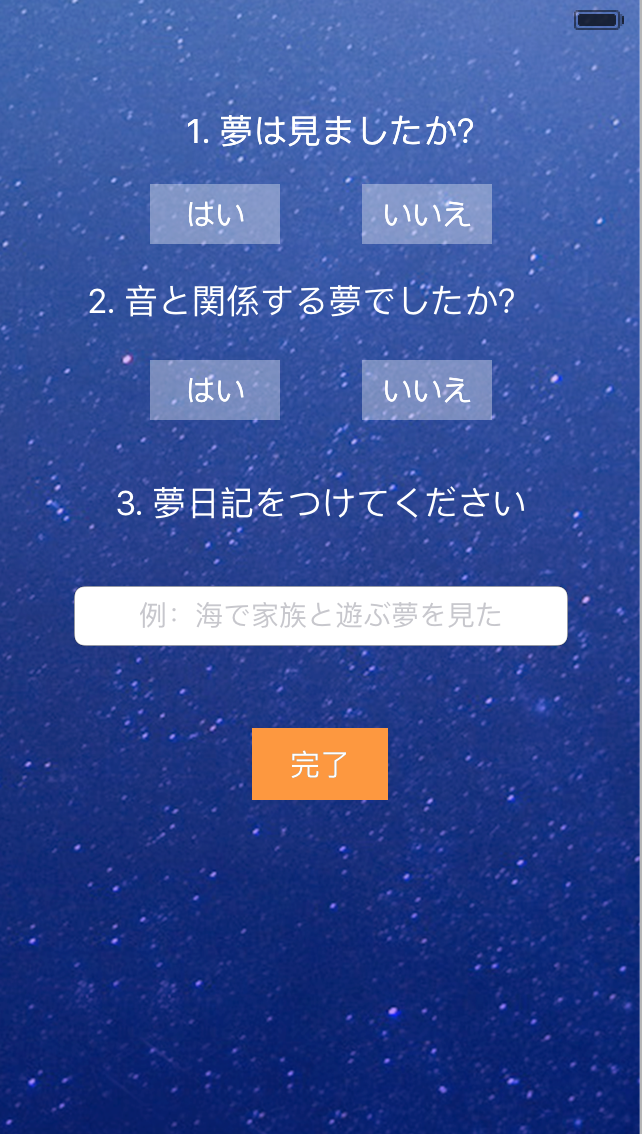
\includegraphics[height=90mm]{eps/AppDiary.eps}
  \end{center}
  \caption{上にスワイプで上下移動}
  \label{le05}
 \end{minipage}
 \begin{minipage}{0.45\hsize}
 \end{minipage}
\end{figure}

\section{システム概要}
\subsection{センシングの方法とその正確性}
 DreamScapeを使うとき、ユーザーは事前に音声を登録してもらうことが必要となる。DreamScapeに適している音声と適さない音声がある。人の声、特に喋りかけてくるような内容の音声は、ユーザーを起こしてしまう可能性がある。適している音は繰り返しある環境下で聞いていた音である。例えば、旅で聞いていた曲、好きな映画のサウンドトラック、最寄り駅の音楽、特的の誰かと良く聞いていた音楽などが効果的だ。
 アプリを初めて起動するとこのような手順が表示される。自動ロック機能をOFFにして、音量は1〜3に設定してもらう。 次にユーザーが登録した音楽が流れる。流れている最中はユーザーにできるだけ思い出の中の空間、香り、音をの細部をまで思い出して、気持ちを落ちつかせてもらう。ユーザーは寝る前にアプリを起動してスタートボタンを押し、起動させたままスクリーンを伏せて枕の横に置く。20〜30分間後にDreamScapeの加速度が起動をし、一晩中ユーザーの体動のモニタリングが行われ、REM睡眠を検知すると音楽がなる。
 起床後、ユーザーは起床すると夢の内容を忘れないように日記に投稿する。